% ============================================================
%  Preparatório OBI — Aula 03
%  Fila (Queue) e Fila de Prioridade (Priority Queue)
%  Grupo: GEMA
%  Compilar: pdflatex aula03_queue.tex  (2x para refs)
% ============================================================
\documentclass[aspectratio=169,11pt]{beamer}

\usetheme{Madrid}
\usecolortheme{default}

% ── Pacotes ───────────────────────────────────────────────
\usepackage[utf8]{inputenc}
\usepackage[T1]{fontenc}
\usepackage[english]{babel}
\usepackage{graphicx}
\usepackage{listings}
\usepackage{xcolor}
\usepackage{tikz}
\usepackage{amsmath}
\usepackage{tcolorbox}
\usepackage{array}
\usepackage{booktabs}
\usepackage{adjustbox}
\tcbuselibrary{skins,breakable,listings}
\usetikzlibrary{arrows.meta,shapes,positioning,fit,calc,
                decorations.pathreplacing,backgrounds}

% ── Margens e listas ──────────────────────────────────────
\setbeamersize{text margin left=5mm,text margin right=5mm}
\setlength{\leftmargini}{1.2em}
\setlength{\leftmarginii}{1.0em}
\setbeamertemplate{itemize/enumerate body begin}{\small}

% ── Paleta de cores ───────────────────────────────────────
\definecolor{gemaBlue}   {RGB}{13,  43,  90}
\definecolor{gemaCyan}   {RGB}{0,  170, 210}
\definecolor{gemaRed}    {RGB}{190, 30,  30}
\definecolor{gemaOrange} {RGB}{220, 110,  0}
\definecolor{gemaGold}   {RGB}{180, 130,  0}
\definecolor{codeBack}   {RGB}{22,  27,  34}
\definecolor{codeGreen}  {RGB}{80,  200, 120}
\definecolor{codeBlue}   {RGB}{121, 192, 255}
\definecolor{codeYellow} {RGB}{255, 210,  70}
\definecolor{codeOrange} {RGB}{255, 160,  60}
\definecolor{alertYellow}{RGB}{255, 243, 176}
\definecolor{alertBorder}{RGB}{160, 110,   0}
\definecolor{queueColor} {RGB}{0,  140, 180}
\definecolor{pqColor}    {RGB}{140,  0, 180}
\definecolor{nodeGreen}  {RGB}{30,  150,  80}

% ── Cores Beamer ──────────────────────────────────────────
\setbeamercolor{palette primary}    {bg=gemaBlue,fg=white}
\setbeamercolor{palette secondary}  {bg=gemaBlue!85,fg=white}
\setbeamercolor{palette tertiary}   {bg=gemaBlue!65,fg=white}
\setbeamercolor{palette quaternary} {bg=gemaBlue,fg=white}
\setbeamercolor{structure}          {fg=gemaBlue}
\setbeamercolor{frametitle}         {fg=white,bg=gemaBlue}
\setbeamercolor{block title}        {fg=white,bg=gemaBlue}
\setbeamercolor{block body}         {fg=black,bg=gemaBlue!7}
\setbeamercolor{block title alerted}{fg=white,bg=gemaRed}
\setbeamercolor{block body alerted} {fg=black,bg=gemaRed!8}
\setbeamercolor{block title example}{fg=white,bg=gemaCyan!75!black}
\setbeamercolor{block body example} {fg=black,bg=gemaCyan!10}
\setbeamercolor{itemize item}       {fg=gemaCyan!70!black}
\setbeamercolor{itemize subitem}    {fg=gemaBlue!60}

\setbeamerfont{frametitle}{size=\large,series=\bfseries}
\setbeamerfont{title}     {size=\LARGE,series=\bfseries}
\setbeamertemplate{navigation symbols}{}

% ── Rodapé ────────────────────────────────────────────────
\setbeamertemplate{footline}{%
  \leavevmode\hbox{%
    \begin{beamercolorbox}[wd=.33\paperwidth,ht=3ex,dp=1.5ex,center]{palette secondary}
      \footnotesize GEMA
    \end{beamercolorbox}%
    \begin{beamercolorbox}[wd=.34\paperwidth,ht=3ex,dp=1.5ex,center]{palette primary}
      \footnotesize Preparatorio OBI --- Aula 03: Queue
    \end{beamercolorbox}%
    \begin{beamercolorbox}[wd=.33\paperwidth,ht=3ex,dp=1.5ex,right]{palette secondary}
      \footnotesize \insertframenumber/\inserttotalframenumber\hspace{2mm}
    \end{beamercolorbox}%
  }%
}

% ── Estilo de código C++ ──────────────────────────────────
\lstdefinestyle{cppstyle}{
  language=C++,
  backgroundcolor=\color{codeBack},
  basicstyle=\ttfamily\footnotesize\color{white},
  keywordstyle=\color{codeBlue}\bfseries,
  stringstyle=\color{codeOrange},
  commentstyle=\color{codeGreen}\itshape,
  numberstyle=\tiny\color{gray!60},
  identifierstyle=\color{white},
  morekeywords={queue,priority_queue,stack,vector,pair,greater,bool,auto,long},
  emph={push,pop,front,back,top,empty,size,cin,cout,endl,min,max,make_pair},
  emphstyle=\color{codeYellow}\bfseries,
  numbers=left,
  numbersep=6pt,
  frame=none,
  tabsize=4,
  showstringspaces=false,
  breaklines=true,
  columns=flexible,
  keepspaces=true,
  xleftmargin=12pt,
  aboveskip=0pt,
  belowskip=0pt,
}

\lstdefinestyle{cppsmall}{
  style=cppstyle,
  basicstyle=\ttfamily\tiny\color{white},
  numberstyle=\tiny\color{gray!50},
  numbersep=4pt,
  xleftmargin=8pt,
  lineskip=-0.5pt,
}

% ── Caixas ────────────────────────────────────────────────
\tcbset{
  before skip=2pt, after skip=2pt, boxsep=1pt,
  caixaBase/.style={
    enhanced,arc=5pt,boxrule=1pt,
    left=4pt,right=4pt,top=3pt,bottom=3pt,
    fonttitle=\bfseries\small,
  },
  caixaAzul/.style={caixaBase,
    colback=gemaBlue!6,colframe=gemaBlue},
  caixaVerde/.style={caixaBase,
    colback=codeGreen!8,colframe=codeGreen!55!black,
    fonttitle=\bfseries\small\color{codeGreen!35!black}},
  caixaVermelho/.style={caixaBase,
    colback=gemaRed!8,colframe=gemaRed,
    fonttitle=\bfseries\small\color{gemaRed!80!black}},
  caixaLaranja/.style={caixaBase,
    colback=gemaOrange!8,colframe=gemaOrange,
    fonttitle=\bfseries\small\color{gemaOrange!80!black}},
  caixaRoxa/.style={caixaBase,
    colback=pqColor!8,colframe=pqColor!70,
    fonttitle=\bfseries\small\color{pqColor!70!black}},
  caixaAmarelo/.style={caixaBase,
    colback=alertYellow,colframe=alertBorder,
    fonttitle=\bfseries\small\color{alertBorder}},
  caixaCodigo/.style={
    enhanced,arc=5pt,boxrule=1pt,
    colback=codeBack,colframe=gemaCyan!45,
    left=1pt,right=1pt,top=1pt,bottom=1pt},
}

% ── Metadados ─────────────────────────────────────────────
\title[Aula 03 --- Queue]{Fila e Fila de Prioridade}
\subtitle{Preparatorio OBI --- Aula 03}
\author[GEMA]{Grupo de Extensao em Maratonas de Programacao}
\institute{GEMA}
\date{2025}

% =============================================================
\begin{document}
% =============================================================

% ─────────────────────────────────────────────────────────────
%  SLIDE DE TÍTULO
% ─────────────────────────────────────────────────────────────
{
\setbeamertemplate{footline}{}
\begin{frame}[noframenumbering]
  \begin{columns}[c]
    \column{0.60\textwidth}
      \vspace{0.3cm}
      {\fontsize{18}{22}\selectfont\bfseries\color{gemaBlue}
        Fila (Queue) e Fila de Prioridade\par}
      \vspace{0.2cm}
      {\large\color{gemaCyan} Preparatorio OBI --- Aula 03\par}
      \vspace{0.1cm}
      {\small\color{gray} Estruturas de Dados $\cdot$ OBI $\cdot$ ICPC\par}
      \vspace{0.45cm}
      \begin{tcolorbox}[caixaAzul,title={}]
        \footnotesize
        \textbf{Aula anterior:} Stack (Pilha) --- LIFO\\[2pt]
        \textbf{Hoje:} Queue (FIFO) e Priority Queue (Heap)\\[2pt]
        \textbf{Pre-req:} Arrays, C++ basico, Stack
      \end{tcolorbox}
    \column{0.38\textwidth}
      \centering
      
\includegraphics[width=0.50\linewidth]{logo.png}\\[0.35cm]
      
\includegraphics[width=0.50\linewidth]{logo_obi.png}
  \end{columns}
\end{frame}
}

% ─────────────────────────────────────────────────────────────
%  AGENDA
% ─────────────────────────────────────────────────────────────
\begin{frame}{Agenda}
  \begin{columns}[t]
    \column{0.47\textwidth}
      \begin{block}{Parte 1 --- Queue (Fila)}
        \begin{enumerate}\small
          \item Revisao: Stack vs Queue
          \item Conceito FIFO
          \item Operacoes: push, pop, front
          \item Implementacao C++ (STL)
          \item Complexidade
          \item Aplicacoes: BFS e simulacoes
        \end{enumerate}
      \end{block}
    \column{0.47\textwidth}
      \begin{block}{Parte 2 --- Priority Queue}
        \begin{enumerate}\small
          \item Conceito de heap
          \item Max-heap vs Min-heap
          \item Implementacao C++ (STL)
          \item Complexidade
          \item Dijkstra e agendamento
          \item Comparacao e escolha certa
        \end{enumerate}
      \end{block}
  \end{columns}
  \vspace{0.3cm}
  \begin{tcolorbox}[caixaAmarelo,title={Objetivo da aula}]
    \small Saber \textbf{quando} usar Queue, \textbf{quando} usar Priority Queue
    e \textbf{como} implementar ambas em C++ para problemas da OBI.
  \end{tcolorbox}
\end{frame}

% =============================================================
%  DIVISOR REVISÃO
% =============================================================
{
\setbeamertemplate{footline}{}
\begin{frame}[noframenumbering]
  \centering\vspace{1.0cm}
  {\fontsize{32}{38}\selectfont\bfseries\color{gemaBlue} Revisao}\par
  \vspace{0.3cm}
  {\Large\color{gemaCyan}\bfseries Stack vs.\ Queue}\par
  \vspace{0.2cm}
  {\color{gray}\small LIFO $\times$ FIFO --- a diferenca fundamental}
\end{frame}
}

% ─────────────────────────────────────────────────────────────
%  STACK VS QUEUE — COMPARAÇÃO VISUAL
% ─────────────────────────────────────────────────────────────
\begin{frame}{Stack vs.\ Queue --- Comparacao Visual}
  \centering
  \begin{adjustbox}{max totalsize={0.98\textwidth}{0.72\textheight},center}
  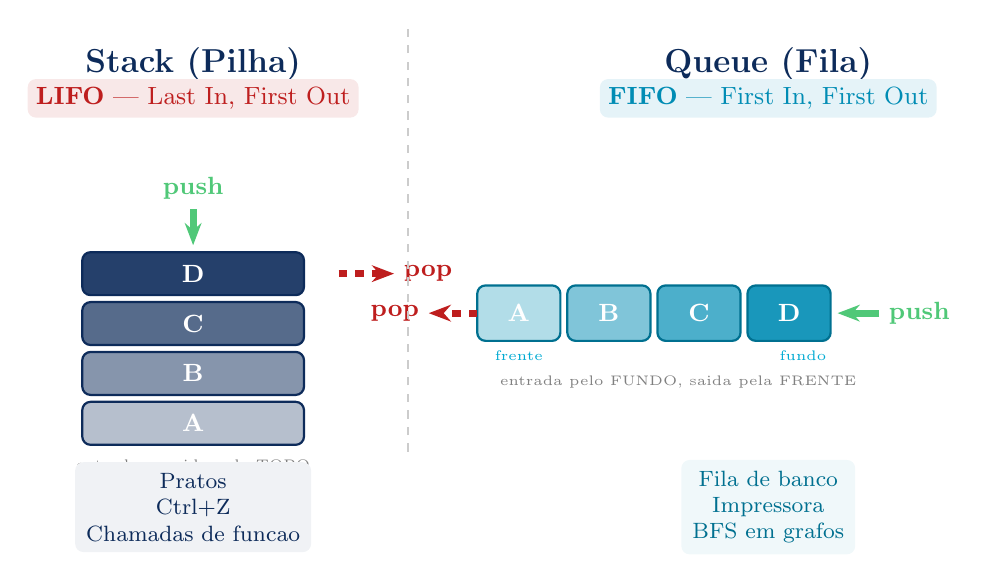
\begin{tikzpicture}[scale=0.88]

    % ════════ STACK (lado esquerdo) ════════
    \node[font=\bfseries\large,gemaBlue] at (2.2,5.5){Stack (Pilha)};
    \node[font=\small,gemaRed,fill=gemaRed!10,rounded corners=3pt,
          inner sep=3pt] at (2.2,5.0){\textbf{LIFO} --- Last In, First Out};

    % blocos empilhados verticalmente
    \foreach \val/\shade/\y in {A/30/0, B/50/0.72, C/70/1.44, D/90/2.16}{
      \draw[fill=gemaBlue!\shade,draw=gemaBlue,rounded corners=3pt,line width=0.8pt]
        (0.6,\y) rectangle (3.8,\y+0.62)
        node[midway,white,font=\bfseries\small]{\val};
    }
    % entrada (topo)
    \draw[-{Stealth[length=8pt]},codeGreen,line width=2.5pt]
      (2.2,3.4)--(2.2,2.88);
    \node[above,codeGreen,font=\bfseries\small] at (2.2,3.4){push};
    % saida (topo)
    \draw[-{Stealth[length=8pt]},gemaRed,line width=2.5pt,dashed]
      (4.3,2.47)--(5.1,2.47);
    \node[right,gemaRed,font=\bfseries\small] at (5.1,2.47){pop};
    % label topo
    \node[gemaCyan,font=\small\bfseries,right] at (4.3,2.47){};
    \node[font=\tiny,gray] at (2.2,-0.3){entrada = saida pelo TOPO};

    % ════════ QUEUE (lado direito) ════════
    \node[font=\bfseries\large,gemaBlue] at (10.5,5.5){Queue (Fila)};
    \node[font=\small,queueColor,fill=queueColor!10,rounded corners=3pt,
          inner sep=3pt] at (10.5,5.0){\textbf{FIFO} --- First In, First Out};

    % blocos horizontais
    \foreach \val/\shade/\x in {A/30/6.3, B/50/7.6, C/70/8.9, D/90/10.2}{
      \draw[fill=queueColor!\shade,draw=queueColor!80!black,rounded corners=3pt,
            line width=0.8pt]
        (\x,1.5) rectangle (\x+1.2,2.3)
        node[midway,white,font=\bfseries\small]{\val};
    }
    % entrada (direita — fundo)
    \draw[-{Stealth[length=8pt]},codeGreen,line width=2.5pt]
      (12.1,1.9)--(11.5,1.9);
    \node[right,codeGreen,font=\bfseries\small] at (12.1,1.9){push};
    % saida (esquerda — frente)
    \draw[-{Stealth[length=8pt]},gemaRed,line width=2.5pt,dashed]
      (6.3,1.9)--(5.6,1.9);
    \node[left,gemaRed,font=\bfseries\small] at (5.6,1.9){pop};
    % labels frente/fundo
    \node[font=\tiny,gemaCyan,below] at (6.9,1.5){frente};
    \node[font=\tiny,gemaCyan,below] at (11.0,1.5){fundo};
    % label
    \node[font=\tiny,gray] at (9.2,0.9){entrada pelo FUNDO, saida pela FRENTE};

    % linha separadora
    \draw[gray!40,dashed,line width=1pt] (5.3,-0.1)--(5.3,6.0);

    % analogias
    \node[font=\footnotesize,gemaBlue,fill=gemaBlue!6,rounded corners=3pt,
          inner sep=4pt,align=center] at (2.2,-0.9)
      {Pratos \\ Ctrl+Z \\ Chamadas de funcao};
    \node[font=\footnotesize,queueColor!80!black,fill=queueColor!6,
          rounded corners=3pt,inner sep=4pt,align=center] at (10.5,-0.9)
      {Fila de banco \\ Impressora \\ BFS em grafos};

  \end{tikzpicture}
  \end{adjustbox}
\end{frame}

% =============================================================
%  DIVISOR PARTE 1
% =============================================================
{
\setbeamertemplate{footline}{}
\begin{frame}[noframenumbering]
  \centering\vspace{1.2cm}
  {\fontsize{40}{48}\selectfont\bfseries\color{gemaBlue} 1}\par
  \vspace{0.3cm}
  {\Large\color{gemaCyan}\bfseries Queue (Fila)}\par
  \vspace{0.2cm}
  {\color{gray}\small FIFO $\cdot$ Operacoes $\cdot$ Implementacao $\cdot$ BFS}
\end{frame}
}

% ─────────────────────────────────────────────────────────────
%  CONCEITO DE FILA
% ─────────────────────────────────────────────────────────────
\begin{frame}{O que e uma Queue (Fila)?}
  \begin{columns}[c]
    \column{0.50\textwidth}
      \begin{tcolorbox}[caixaAzul,title={Definicao}]
        Uma \textbf{fila} e uma estrutura linear onde o
        \textbf{primeiro elemento inserido} e o
        \textbf{primeiro a ser removido}.
      \end{tcolorbox}
      \vspace{0.2cm}
      \begin{tcolorbox}[caixaLaranja,title={Regra de Ouro --- FIFO}]
        \textbf{F}irst \textbf{I}n, \textbf{F}irst \textbf{O}ut\\[3pt]
        Entrada pelo \textbf{fundo}, saida pela \textbf{frente}.
      \end{tcolorbox}
      \vspace{0.2cm}
      \textbf{Analogias:}
      \begin{itemize}\small
        \item Fila de banco ou supermercado
        \item Fila de impressora
        \item Chamadas de suporte tecnico
        \item Passageiros embarcando no onibus
      \end{itemize}
    \column{0.48\textwidth}
      \centering
      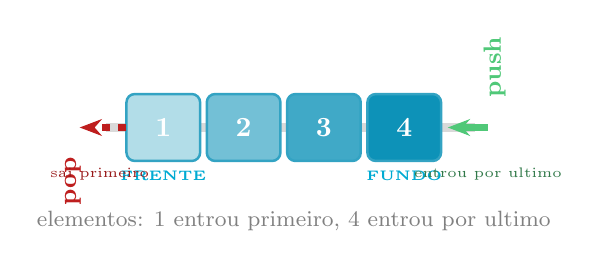
\begin{tikzpicture}[scale=0.85]
        % Trilho
        \draw[gray!30,line width=3pt] (0,1.0)--(5.5,1.0);
        % Blocos
        \foreach \val/\shade/\x in {1/30/0.3, 2/55/1.5, 3/75/2.7, 4/95/3.9}{
          \draw[fill=queueColor!\shade,draw=queueColor!80,rounded corners=3pt,
                line width=0.9pt]
            (\x,0.5) rectangle (\x+1.1,1.5)
            node[midway,white,font=\bfseries]{\val};
        }
        % Seta entrada (fundo, direita)
        \draw[-{Stealth[length=8pt]},codeGreen,line width=2.5pt]
          (5.7,1.0)--(5.1,1.0);
        \node[right,codeGreen,font=\bfseries\small,rotate=90] at (5.8,1.3){push};

        % Seta saida (frente, esquerda)
        \draw[-{Stealth[length=8pt]},gemaRed,line width=2.5pt,dashed]
          (0.3,1.0)--(-0.4,1.0);
        \node[left,gemaRed,font=\bfseries\small,rotate=90] at (-0.5,0.7){pop};

        % Labels
        \node[gemaCyan,font=\tiny\bfseries,below] at (0.85,0.5){FRENTE};
        \node[gemaCyan,font=\tiny\bfseries,below] at (4.45,0.5){FUNDO};

        % Numeros de entrada
        \node[codeGreen!60!black,font=\tiny] at (5.7,0.3){entrou por ultimo};
        \node[gemaRed!80!black,font=\tiny] at (-0.1,0.3){sai primeiro};

        % Label principal
        \node[font=\footnotesize,gray,below] at (2.8,-0.1)
          {elementos: 1 entrou primeiro, 4 entrou por ultimo};
      \end{tikzpicture}
      \vspace{0.25cm}
      \begin{tcolorbox}[caixaVerde,title={Chave}]
        \footnotesize
        Quem chegou \textbf{primeiro} na fila
        e o \textbf{primeiro} a ser atendido.
      \end{tcolorbox}
  \end{columns}
\end{frame}

% ─────────────────────────────────────────────────────────────
%  OPERAÇÕES DA FILA
% ─────────────────────────────────────────────────────────────
\begin{frame}{Operacoes da Queue}
  \begin{columns}[t]
    \column{0.31\textwidth}
      \begin{exampleblock}{push(x) / enqueue}
        \small
        Insere \texttt{x} no \textbf{fundo}.\\[4pt]
        \textbf{O(1)} sempre.\\[4pt]
        Nunca falha por si so.
      \end{exampleblock}
    \column{0.31\textwidth}
      \begin{alertblock}{pop() / dequeue}
        \small
        Remove a \textbf{frente}.\\[4pt]
        \textbf{O(1)}\\[4pt]
        \textcolor{gemaRed}{\textbf{CRASH se vazia!}}
      \end{alertblock}
    \column{0.31\textwidth}
      \begin{block}{front()}
        \small
        Le a frente sem remover.\\[4pt]
        \textbf{O(1)}\\[4pt]
        \textcolor{gemaRed}{\textbf{CRASH se vazia!}}
      \end{block}
  \end{columns}
  \vspace{0.2cm}
  \begin{columns}[t]
    \column{0.31\textwidth}
      \begin{block}{back()}
        \small
        Le o fundo sem remover.\\[4pt]
        \textbf{O(1)}
      \end{block}
    \column{0.31\textwidth}
      \begin{block}{empty() / size()}
        \small
        Verifica se vazia.\\
        Retorna o tamanho.\\[4pt]
        \textbf{O(1)} ambos.
      \end{block}
    \column{0.31\textwidth}
      \begin{tcolorbox}[caixaVerde,title={Dica de Prova}]
        \small
        Sempre verifique\\
        \texttt{!q.empty()} antes\\
        de \texttt{front()} e \texttt{pop()}.
      \end{tcolorbox}
  \end{columns}
  \vspace{0.18cm}
  \begin{tcolorbox}[caixaAzul,title={Diferenca critica: Queue vs Stack}]
    \centering\small
    \begin{tabular}{lll}
      \toprule
      & \textbf{Stack} & \textbf{Queue}\\
      \midrule
      Inserir & \texttt{push} $\to$ topo & \texttt{push} $\to$ fundo\\
      Remover & \texttt{pop} do topo & \texttt{pop} da frente\\
      Ler     & \texttt{top()} & \texttt{front()}\\
      \bottomrule
    \end{tabular}
  \end{tcolorbox}
\end{frame}

% ─────────────────────────────────────────────────────────────
%  QUEUE PASSO A PASSO
% ─────────────────────────────────────────────────────────────
\begin{frame}{Queue --- Passo a Passo}
  \centering
  \begin{adjustbox}{max totalsize={0.98\textwidth}{0.74\textheight},center}
  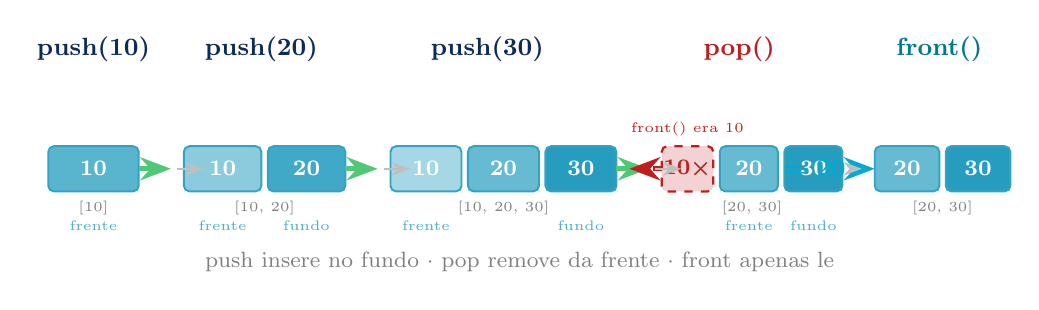
\begin{tikzpicture}[scale=0.82]

    % ── Helper: bloco horizontal ──────────────────────────
    % Macro: caixa em (x,y) com largura 1.1 e altura 0.65
    % usaremos tikz direto

    % ─── Estado 1: push(10) ───────────────────────────────
    \node[font=\bfseries\small,gemaBlue] at (0.9,3.2){push(10)};
    \draw[fill=queueColor!65,draw=queueColor!80,rounded corners=2pt,line width=0.7pt]
      (0.2,1.0) rectangle (1.6,1.7) node[midway,white,font=\bfseries\footnotesize]{10};
    \draw[-{Stealth},codeGreen,line width=1.8pt] (1.6,1.35)--(2.1,1.35);
    \node[font=\tiny,gray,below] at (0.9,1.0){[10]};
    \node[font=\tiny,queueColor!70,below] at (0.9,0.7){frente};

    % ─── Estado 2: push(20) ───────────────────────────────
    \node[font=\bfseries\small,gemaBlue] at (3.5,3.2){push(20)};
    \draw[fill=queueColor!45,draw=queueColor!80,rounded corners=2pt,line width=0.7pt]
      (2.3,1.0) rectangle (3.5,1.7) node[midway,white,font=\bfseries\footnotesize]{10};
    \draw[fill=queueColor!75,draw=queueColor!80,rounded corners=2pt,line width=0.7pt]
      (3.6,1.0) rectangle (4.8,1.7) node[midway,white,font=\bfseries\footnotesize]{20};
    \draw[-{Stealth},codeGreen,line width=1.8pt] (4.8,1.35)--(5.3,1.35);
    \node[font=\tiny,gray,below] at (3.55,1.0){[10,\ 20]};
    \node[font=\tiny,queueColor!70,below] at (2.9,0.7){frente};
    \node[font=\tiny,queueColor!70,below] at (4.2,0.7){fundo};

    % ─── Estado 3: push(30) ───────────────────────────────
    \node[font=\bfseries\small,gemaBlue] at (7.0,3.2){push(30)};
    \draw[fill=queueColor!35,draw=queueColor!80,rounded corners=2pt,line width=0.7pt]
      (5.5,1.0) rectangle (6.6,1.7) node[midway,white,font=\bfseries\footnotesize]{10};
    \draw[fill=queueColor!60,draw=queueColor!80,rounded corners=2pt,line width=0.7pt]
      (6.7,1.0) rectangle (7.8,1.7) node[midway,white,font=\bfseries\footnotesize]{20};
    \draw[fill=queueColor!85,draw=queueColor!80,rounded corners=2pt,line width=0.7pt]
      (7.9,1.0) rectangle (9.0,1.7) node[midway,white,font=\bfseries\footnotesize]{30};
    \draw[-{Stealth},codeGreen,line width=1.8pt] (9.0,1.35)--(9.5,1.35);
    \node[font=\tiny,gray,below] at (7.25,1.0){[10,\ 20,\ 30]};
    \node[font=\tiny,queueColor!70,below] at (6.05,0.7){frente};
    \node[font=\tiny,queueColor!70,below] at (8.45,0.7){fundo};

    % ─── Estado 4: pop() ──────────────────────────────────
    \node[font=\bfseries\small,gemaRed] at (10.9,3.2){pop()};
    % 10 saindo (tracejado)
    \draw[fill=gemaRed!20,draw=gemaRed,rounded corners=2pt,
          line width=0.8pt,dashed]
      (9.7,1.0) rectangle (10.5,1.7)
      node[midway,gemaRed,font=\bfseries\footnotesize]{10\texttimes};
    \draw[-{Stealth},gemaRed,line width=1.8pt,dashed]
      (9.7,1.35)--(9.2,1.35);
    % 20, 30 ficam
    \draw[fill=queueColor!60,draw=queueColor!80,rounded corners=2pt,line width=0.7pt]
      (10.6,1.0) rectangle (11.5,1.7) node[midway,white,font=\bfseries\footnotesize]{20};
    \draw[fill=queueColor!85,draw=queueColor!80,rounded corners=2pt,line width=0.7pt]
      (11.6,1.0) rectangle (12.5,1.7) node[midway,white,font=\bfseries\footnotesize]{30};
    \node[font=\tiny,gray,below] at (11.1,1.0){[20,\ 30]};
    \node[font=\tiny,queueColor!70,below] at (11.05,0.7){frente};
    \node[font=\tiny,queueColor!70,below] at (12.05,0.7){fundo};
    \node[font=\tiny,gemaRed,above] at (10.1,1.7){front() era 10};

    % ─── Estado 5: front() ────────────────────────────────
    \node[font=\bfseries\small,gemaCyan!70!black] at (14.0,3.2){front()};
    \draw[fill=queueColor!60,draw=queueColor!80,rounded corners=2pt,line width=0.7pt]
      (13.0,1.0) rectangle (14.0,1.7) node[midway,white,font=\bfseries\footnotesize]{20};
    \draw[fill=queueColor!85,draw=queueColor!80,rounded corners=2pt,line width=0.7pt]
      (14.1,1.0) rectangle (15.1,1.7) node[midway,white,font=\bfseries\footnotesize]{30};
    \draw[-{Stealth},gemaCyan,line width=1.8pt]
      (12.7,1.35)--(13.0,1.35);
    \node[left,gemaCyan,font=\bfseries\small] at (12.7,1.35){= 20};
    \node[font=\tiny,gray,below] at (14.05,1.0){[20,\ 30]};

    % Setas de transicao entre estados
    \foreach \x in {2.1, 5.3, 9.5}{
      \draw[-{Stealth},gray!50,line width=0.8pt] (\x+0.1,1.35)--(\x+0.5,1.35);
    }
    \draw[-{Stealth},gray!50,line width=0.8pt] (12.6,1.35)--(12.8,1.35);

    % Legenda
    \node[font=\footnotesize,gray] at (7.5,-0.1)
      {push insere no fundo $\cdot$ pop remove da frente $\cdot$ front apenas le};

  \end{tikzpicture}
  \end{adjustbox}
\end{frame}

% ─────────────────────────────────────────────────────────────
%  IMPLEMENTAÇÃO STL — QUEUE
% ─────────────────────────────────────────────────────────────
\begin{frame}[fragile,shrink=5]{Implementacao em C++ --- Queue STL}
  \begin{columns}[t]
    \column{0.60\textwidth}
      \begin{tcolorbox}[caixaCodigo]
        \begin{lstlisting}[style=cppstyle]
#include <bits/stdc++.h>
using namespace std;

int main() {
    queue<int> q;  // fila de inteiros

    q.push(10);    // insere no fundo: [10]
    q.push(20);    // insere no fundo: [10, 20]
    q.push(30);    // insere no fundo: [10, 20, 30]

    // SEMPRE verifica antes de acessar!
    cout << q.front() << "\n"; // 10 (frente)
    cout << q.back()  << "\n"; // 30 (fundo)

    q.pop();   // remove da frente -> [20, 30]
    cout << q.front() << "\n"; // 20

    cout << q.size() << "\n";  // 2

    while (!q.empty()) {
        cout << q.front() << " "; // 20 30
        q.pop();
    }
    return 0;
}
        \end{lstlisting}
      \end{tcolorbox}
    \column{0.37\textwidth}
      \vspace{0.1cm}
      \begin{tcolorbox}[caixaAzul,title={Resumo STL}]
        \footnotesize
        \begin{tabular}{@{}ll@{}}
          \texttt{push(x)}  & insere no fundo\\[3pt]
          \texttt{pop()}    & remove da frente\\[3pt]
          \texttt{front()}  & le a frente\\[3pt]
          \texttt{back()}   & le o fundo\\[3pt]
          \texttt{empty()}  & esta vazia?\\[3pt]
          \texttt{size()}   & quantos?\\
        \end{tabular}
      \end{tcolorbox}
      \vspace{0.2cm}
      \begin{tcolorbox}[caixaVermelho,title={Atencao}]
        \footnotesize
        \textbf{Nao existe} \texttt{top()} na queue!\\[3pt]
        Use \texttt{front()} para ler\\
        o primeiro elemento.\\[3pt]
        \texttt{pop()} remove\\
        \textbf{sem retornar} o valor.
      \end{tcolorbox}
  \end{columns}
\end{frame}

% ─────────────────────────────────────────────────────────────
%  COMPLEXIDADE — QUEUE
% ─────────────────────────────────────────────────────────────
\begin{frame}{Complexidade da Queue}
  \begin{columns}[c]
    \column{0.55\textwidth}
      \begin{tcolorbox}[caixaAzul,title={Tabela de Complexidade}]
        \centering\small
        \begin{tabular}{lcc}
          \toprule
          \textbf{Operacao} & \textbf{Tempo} & \textbf{Espaco}\\
          \midrule
          \texttt{push(x)}  & O(1) & O(1)\\
          \texttt{pop()}    & O(1) & O(1)\\
          \texttt{front()}  & O(1) & O(1)\\
          \texttt{back()}   & O(1) & O(1)\\
          \texttt{empty()}  & O(1) & O(1)\\
          \texttt{size()}   & O(1) & O(1)\\
          \midrule
          \textbf{Espaco total} & --- & O(n)\\
          \bottomrule
        \end{tabular}
      \end{tcolorbox}
      \vspace{0.2cm}
      \begin{tcolorbox}[caixaVerde,title={Por que tudo e O(1)?}]
        \small
        A STL implementa a queue internamente com
        um \textbf{deque} (fila dupla), que permite
        insercao e remocao eficiente em ambas as extremidades.
      \end{tcolorbox}
    \column{0.42\textwidth}
      \begin{tcolorbox}[caixaAmarelo,title={Comparacao}]
        \small
        \begin{tabular}{lcc}
          \toprule
          & \textbf{Stack} & \textbf{Queue}\\
          \midrule
          push & O(1) & O(1)\\
          pop  & O(1) & O(1)\\
          peek & O(1) & O(1)\\
          \bottomrule
        \end{tabular}\\[6pt]
        Ambas sao \textbf{igualmente eficientes}!\\
        A diferenca e \textbf{comportamental}:\\
        LIFO vs FIFO.
      \end{tcolorbox}
      \vspace{0.2cm}
      \begin{tcolorbox}[caixaVermelho,title={Cuidado}]
        \small
        A queue da STL \textbf{nao} permite:
        \begin{itemize}\footnotesize
          \item Acesso por indice (\texttt{q[i]})
          \item Iterar sem destruir
          \item Pesquisa por valor
        \end{itemize}
      \end{tcolorbox}
  \end{columns}
\end{frame}

% ─────────────────────────────────────────────────────────────
%  BFS — APLICAÇÃO DA QUEUE
% ─────────────────────────────────────────────────────────────
\begin{frame}{Aplicacao Classica --- BFS (Busca em Largura)}
  \begin{columns}[c]
    \column{0.48\textwidth}
      \begin{tcolorbox}[caixaAzul,title={O que e BFS?}]
        \small
        Explora um grafo \textbf{nivel por nivel}:
        primeiro todos os vizinhos do inicio,
        depois os vizinhos dos vizinhos, etc.\\[4pt]
        \textbf{Queue e essencial:} garante que os
        nos sao visitados na ordem correta (FIFO).
      \end{tcolorbox}
      \vspace{0.15cm}
      \textbf{Algoritmo:}
      \begin{enumerate}\small
        \item Insere o no inicial na queue
        \item Enquanto a queue nao esta vazia:
        \begin{itemize}\footnotesize
          \item Retira o no da frente
          \item Marca como visitado
          \item Insere todos os vizinhos nao visitados
        \end{itemize}
      \end{enumerate}
    \column{0.50\textwidth}
      \centering
      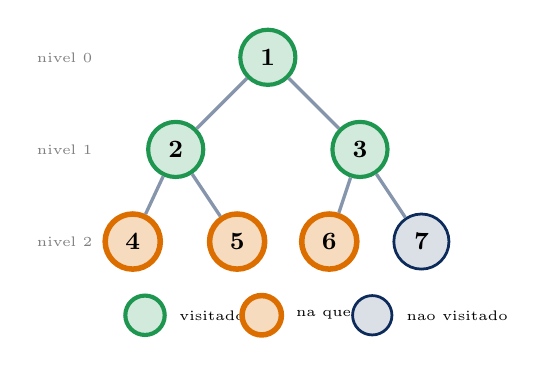
\begin{tikzpicture}[scale=0.78,
          no/.style={circle,draw=gemaBlue,fill=gemaBlue!15,
                     minimum size=7mm,font=\bfseries\small,line width=1pt},
          vis/.style={circle,draw=nodeGreen,fill=nodeGreen!20,
                      minimum size=7mm,font=\bfseries\small,line width=1.5pt},
          fron/.style={circle,draw=gemaOrange,fill=gemaOrange!25,
                       minimum size=7mm,font=\bfseries\small,line width=2pt},
        ]
        % Nos
        \node[vis]  (1) at (2.5,3.5) {1};
        \node[vis]  (2) at (1.0,2.0) {2};
        \node[vis]  (3) at (4.0,2.0) {3};
        \node[fron] (4) at (0.3,0.5) {4};
        \node[fron] (5) at (2.0,0.5) {5};
        \node[fron] (6) at (3.5,0.5) {6};
        \node[no]   (7) at (5.0,0.5) {7};
        % Arestas
        \foreach \a/\b in {1/2,1/3,2/4,2/5,3/6,3/7}{
          \draw[gemaBlue!50,line width=1.2pt] (\a)--(\b);
        }
        % Legenda
        \node[vis,minimum size=5mm] at (0.5,-0.7){};
        \node[font=\tiny,right] at (0.9,-0.7){visitado};
        \node[fron,minimum size=5mm] at (2.4,-0.7){};
        \node[font=\tiny,right] at (2.8,-0.7){na queue};
        \node[no,minimum size=5mm] at (4.2,-0.7){};
        \node[font=\tiny,right] at (4.6,-0.7){nao visitado};

        % Niveis
        \node[font=\tiny,gray,left] at (-0.2,3.5){nivel 0};
        \node[font=\tiny,gray,left] at (-0.2,2.0){nivel 1};
        \node[font=\tiny,gray,left] at (-0.2,0.5){nivel 2};
      \end{tikzpicture}
      \vspace{0.05cm}
      \begin{tcolorbox}[caixaVerde,title={Estado atual}]
        \footnotesize
        Queue: \texttt{[4, 5, 6]}\\
        Visitados: \texttt{1, 2, 3}\\
        Proximos: processar nivel 2
      \end{tcolorbox}
  \end{columns}
\end{frame}

% ─────────────────────────────────────────────────────────────
%  BFS — CÓDIGO
% ─────────────────────────────────────────────────────────────
\begin{frame}[fragile,shrink=8]{BFS em Grafo --- Codigo Completo}
  \begin{columns}[t]
    \column{0.58\textwidth}
      \begin{tcolorbox}[caixaCodigo]
        \begin{lstlisting}[style=cppsmall]
#include <bits/stdc++.h>
using namespace std;

// BFS a partir do no 'inicio' em grafo com N nos
void bfs(int inicio, int N,
         vector<vector<int>>& adj) {

    vector<bool> visitado(N+1, false);
    vector<int>  dist(N+1, -1);
    queue<int> q;

    // passo 1: insere no inicial
    q.push(inicio);
    visitado[inicio] = true;
    dist[inicio] = 0;

    while (!q.empty()) {
        int v = q.front(); // pega a frente
        q.pop();           // remove da fila

        cout << "Visitando no " << v
             << " (dist=" << dist[v] << ")\n";

        // explora vizinhos
        for (int u : adj[v]) {
            if (!visitado[u]) {
                visitado[u] = true;
                dist[u] = dist[v] + 1;
                q.push(u); // insere no fundo
            }
        }
    }
}
        \end{lstlisting}
      \end{tcolorbox}
    \column{0.39\textwidth}
      \vspace{0.1cm}
      \begin{tcolorbox}[caixaAzul,title={Por que Queue?}]
        \footnotesize
        A queue garante que nos visitamos\\
        \textbf{nivel por nivel}.\\[4pt]
        Se usassemos Stack (LIFO),\\
        fariamos DFS (busca em\\
        profundidade), nao BFS!
      \end{tcolorbox}
      \vspace{0.2cm}
      \begin{tcolorbox}[caixaVerde,title={Complexidade BFS}]
        \footnotesize
        \textbf{Tempo:} O(V + E)\\
        V = vertices, E = arestas\\[4pt]
        \textbf{Espaco:} O(V)\\
        (queue + vetor visitado)\\[4pt]
        \textbf{Garante:} distancia\\
        minima em grafos sem peso.
      \end{tcolorbox}
      \vspace{0.2cm}
      \begin{tcolorbox}[caixaAmarelo,title={Aplicacoes na OBI}]
        \footnotesize
        Menor caminho em labirinto\\
        Menor numero de movimentos\\
        Nivel de contaminacao\\
        Propagacao em grade
      \end{tcolorbox}
  \end{columns}
\end{frame}

% =============================================================
%  DIVISOR PARTE 2
% =============================================================
{
\setbeamertemplate{footline}{}
\begin{frame}[noframenumbering]
  \centering\vspace{1.2cm}
  {\fontsize{40}{48}\selectfont\bfseries\color{gemaBlue} 2}\par
  \vspace{0.3cm}
  {\Large\color{pqColor}\bfseries Fila de Prioridade}\par
  \vspace{0.2cm}
  {\color{gray}\small Heap $\cdot$ Max/Min $\cdot$ Dijkstra $\cdot$ Agendamento}
\end{frame}
}

% ─────────────────────────────────────────────────────────────
%  INTRODUÇÃO — PRIORITY QUEUE
% ─────────────────────────────────────────────────────────────
\begin{frame}{Introducao --- Fila de Prioridade}
  \begin{columns}[c]
    \column{0.50\textwidth}
      \begin{tcolorbox}[caixaRoxa,title={Problema com Queue simples}]
        \small
        Em uma fila normal, o primeiro a entrar e o
        primeiro a sair. Mas e se precisarmos sempre
        atender o \textbf{elemento mais importante}
        independente da ordem de chegada?
      \end{tcolorbox}
      \vspace{0.2cm}
      \begin{tcolorbox}[caixaAzul,title={Solucao: Priority Queue}]
        \small
        Uma \textbf{fila de prioridade} e uma estrutura
        onde cada elemento tem uma \textbf{prioridade}.
        O elemento com a \textbf{maior prioridade}
        (ou menor, dependendo da configuracao)
        e sempre o primeiro a sair.
      \end{tcolorbox}
      \vspace{0.2cm}
      \textbf{Analogias:}
      \begin{itemize}\small
        \item Fila de emergencia no hospital
        \item Servidor processando tarefa mais urgente
        \item Algoritmo de Dijkstra (menor distancia)
      \end{itemize}
    \column{0.48\textwidth}
      \centering
      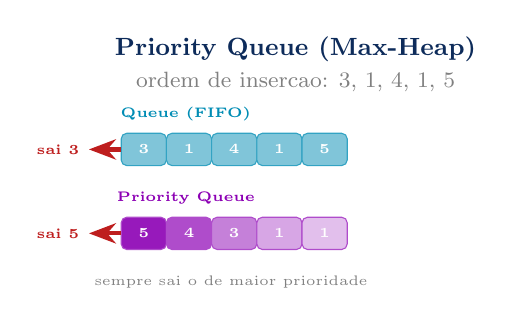
\begin{tikzpicture}[scale=0.82]
        % Fila de prioridade — visualizacao heap
        \node[font=\bfseries\small,gemaBlue] at (2.5,4.0)
          {Priority Queue (Max-Heap)};

        % Comparacao: queue vs pq
        \node[font=\footnotesize,gray] at (2.5,3.5){ordem de insercao: 3, 1, 4, 1, 5};

        % Queue normal
        \node[font=\tiny\bfseries,queueColor] at (0.8,3.0){Queue (FIFO)};
        \foreach \val/\x in {3/0.0, 1/0.7, 4/1.4, 1/2.1, 5/2.8}{
          \draw[fill=queueColor!50,draw=queueColor!80,rounded corners=2pt]
            (\x-0.2,2.2) rectangle (\x+0.5,2.7)
            node[midway,white,font=\tiny\bfseries]{\val};
        }
        \draw[-{Stealth},gemaRed,line width=1.5pt]
          (-0.2,2.45)--(-0.7,2.45);
        \node[left,gemaRed,font=\tiny\bfseries] at (-0.7,2.45){sai 3};

        % Priority Queue
        \node[font=\tiny\bfseries,pqColor] at (0.8,1.7){Priority Queue};
        \foreach \val/\shade/\x in {5/90/0.0, 4/70/0.7, 3/50/1.4, 1/35/2.1, 1/25/2.8}{
          \draw[fill=pqColor!\shade,draw=pqColor!70,rounded corners=2pt]
            (\x-0.2,0.9) rectangle (\x+0.5,1.4)
            node[midway,white,font=\tiny\bfseries]{\val};
        }
        \draw[-{Stealth},gemaRed,line width=1.5pt]
          (-0.2,1.15)--(-0.7,1.15);
        \node[left,gemaRed,font=\tiny\bfseries] at (-0.7,1.15){sai 5};

        \node[font=\tiny,gray] at (1.5,0.4)
          {sempre sai o de maior prioridade};
      \end{tikzpicture}
  \end{columns}
\end{frame}

% ─────────────────────────────────────────────────────────────
%  HEAP — ESTRUTURA INTERNA
% ─────────────────────────────────────────────────────────────
\begin{frame}{Heap --- Estrutura Interna}
  \begin{columns}[c]
    \column{0.50\textwidth}
      \begin{tcolorbox}[caixaAzul,title={O que e um Heap?}]
        \small
        Um \textbf{heap} e uma arvore binaria quase completa
        onde cada no e \textbf{maior (max-heap)} ou
        \textbf{menor (min-heap)} que seus filhos.\\[4pt]
        O elemento da \textbf{raiz} e sempre o maior (ou menor).
      \end{tcolorbox}
      \vspace{0.15cm}
      \begin{tcolorbox}[caixaVermelho,title={Max-Heap}]
        \small Raiz = maior elemento.\\
        \texttt{priority\_queue<int>} na STL.
      \end{tcolorbox}
      \vspace{0.1cm}
      \begin{tcolorbox}[caixaVerde,title={Min-Heap}]
        \small Raiz = menor elemento.\\
        \texttt{priority\_queue<int,vector<int>,greater<int>>}
      \end{tcolorbox}
    \column{0.48\textwidth}
      \centering
      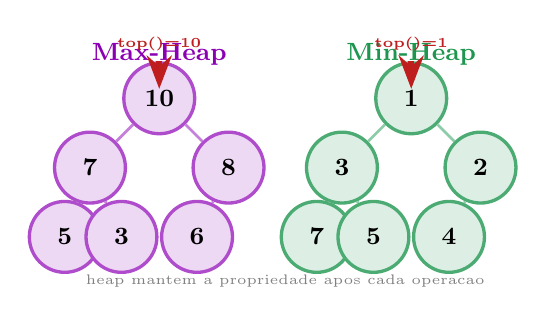
\begin{tikzpicture}[scale=0.80,
          maxno/.style={circle,draw=pqColor!70,fill=pqColor!15,
                        minimum size=9mm,font=\bfseries\small,line width=1.2pt},
          minno/.style={circle,draw=nodeGreen!80,fill=nodeGreen!15,
                        minimum size=9mm,font=\bfseries\small,line width=1.2pt},
        ]
        % MAX-HEAP
        \node[font=\bfseries\small,pqColor] at (1.5,4.5){Max-Heap};
        \node[maxno] (r)  at (1.5,3.8) {10};
        \node[maxno] (l)  at (0.4,2.7) {7};
        \node[maxno] (rr) at (2.6,2.7) {8};
        \node[maxno] (ll) at (0.0,1.6) {5};
        \node[maxno] (lr) at (0.9,1.6) {3};
        \node[maxno] (rl) at (2.1,1.6) {6};
        \draw[pqColor!50,line width=1pt] (r)--(l) (r)--(rr)
          (l)--(ll) (l)--(lr) (rr)--(rl);
        \draw[-{Stealth},gemaRed,line width=2pt] (1.5,4.4)--(1.5,3.95);
        \node[above,gemaRed,font=\tiny\bfseries] at (1.5,4.4){top()=10};

        % MIN-HEAP
        \node[font=\bfseries\small,nodeGreen] at (5.5,4.5){Min-Heap};
        \node[minno] (r2)  at (5.5,3.8) {1};
        \node[minno] (l2)  at (4.4,2.7) {3};
        \node[minno] (rr2) at (6.6,2.7) {2};
        \node[minno] (ll2) at (4.0,1.6) {7};
        \node[minno] (lr2) at (4.9,1.6) {5};
        \node[minno] (rl2) at (6.1,1.6) {4};
        \draw[nodeGreen!50,line width=1pt] (r2)--(l2) (r2)--(rr2)
          (l2)--(ll2) (l2)--(lr2) (rr2)--(rl2);
        \draw[-{Stealth},gemaRed,line width=2pt] (5.5,4.4)--(5.5,3.95);
        \node[above,gemaRed,font=\tiny\bfseries] at (5.5,4.4){top()=1};

        \node[font=\tiny,gray] at (3.5,0.9)
          {heap mantem a propriedade apos cada operacao};
      \end{tikzpicture}
  \end{columns}
\end{frame}

% ─────────────────────────────────────────────────────────────
%  IMPLEMENTAÇÃO — PRIORITY QUEUE
% ─────────────────────────────────────────────────────────────
\begin{frame}[fragile,shrink=6]{Implementacao em C++ --- Priority Queue}
  \begin{columns}[t]
    \column{0.60\textwidth}
      \begin{tcolorbox}[caixaCodigo]
        \begin{lstlisting}[style=cppstyle]
#include <bits/stdc++.h>
using namespace std;

int main() {
    // MAX-HEAP (padrao): maior elemento no topo
    priority_queue<int> maxpq;

    maxpq.push(3);
    maxpq.push(1);
    maxpq.push(4);
    maxpq.push(1);
    maxpq.push(5);

    cout << maxpq.top() << "\n"; // 5 (maior)
    maxpq.pop();
    cout << maxpq.top() << "\n"; // 4

    // MIN-HEAP: menor elemento no topo
    priority_queue<int,
        vector<int>,
        greater<int>> minpq;

    minpq.push(3);
    minpq.push(1);
    minpq.push(4);

    cout << minpq.top() << "\n"; // 1 (menor)
    return 0;
}
        \end{lstlisting}
      \end{tcolorbox}
    \column{0.37\textwidth}
      \vspace{0.05cm}
      \begin{tcolorbox}[caixaRoxa,title={Operacoes PQ}]
        \footnotesize
        \begin{tabular}{@{}ll@{}}
          \texttt{push(x)}  & insere\\[3pt]
          \texttt{pop()}    & remove o topo\\[3pt]
          \texttt{top()}    & le o topo\\[3pt]
          \texttt{empty()}  & esta vazia?\\[3pt]
          \texttt{size()}   & quantos?\\
        \end{tabular}
      \end{tcolorbox}
      \vspace{0.15cm}
      \begin{tcolorbox}[caixaVermelho,title={Atencao}]
        \footnotesize
        \textbf{Nao existe} \texttt{front()} na PQ!\\[3pt]
        Use \texttt{top()} para ver\\
        o elemento de maior\\
        prioridade.\\[3pt]
        \texttt{pop()} remove sem\\
        retornar o valor.
      \end{tcolorbox}
      \vspace{0.15cm}
      \begin{tcolorbox}[caixaVerde,title={Min-heap trick}]
        \footnotesize
        Outra forma de fazer\\
        min-heap:\\
        \texttt{push(-x)} e usar\\
        max-heap padrao.
      \end{tcolorbox}
  \end{columns}
\end{frame}

% ─────────────────────────────────────────────────────────────
%  PQ COM PARES — MUITO COMUM NA OBI
% ─────────────────────────────────────────────────────────────
\begin{frame}[fragile,shrink=6]{Priority Queue com Pares --- Padrao Dijkstra}
  \begin{tcolorbox}[caixaAmarelo,title={Por que usar pares?}]
    \small
    Em Dijkstra e muitos problemas da OBI, precisamos armazenar
    \textbf{(custo, no)} na priority queue. O par e comparado pelo
    primeiro elemento automaticamente.
  \end{tcolorbox}
  \vspace{0.1cm}
  \begin{columns}[t]
    \column{0.58\textwidth}
      \begin{tcolorbox}[caixaCodigo]
        \begin{lstlisting}[style=cppsmall]
#include <bits/stdc++.h>
using namespace std;
typedef pair<int,int> pii;

int main(){
    // Min-heap de pares (custo, no)
    // pair compara pelo 1o elemento primeiro
    priority_queue<pii,
        vector<pii>,
        greater<pii>> pq;

    pq.push({10, 1}); // custo 10, no 1
    pq.push({3,  2}); // custo 3,  no 2
    pq.push({7,  3}); // custo 7,  no 3

    // sai o de MENOR custo primeiro
    while (!pq.empty()) {
        auto [custo, no] = pq.top();
        pq.pop();
        cout << "no=" << no
             << " custo=" << custo << "\n";
    }
    // Saida: no=2 custo=3
    //        no=3 custo=7
    //        no=1 custo=10
}
        \end{lstlisting}
      \end{tcolorbox}
    \column{0.39\textwidth}
      \vspace{0.1cm}
      \begin{tcolorbox}[caixaAzul,title={Declaracoes comuns}]
        \footnotesize
        \textbf{Max-heap de inteiros:}\\
        \texttt{priority\_queue<int> pq;}\\[6pt]
        \textbf{Min-heap de inteiros:}\\
        \texttt{priority\_queue<int,}\\
        \texttt{vector<int>,}\\
        \texttt{greater<int>> pq;}\\[6pt]
        \textbf{Min-heap de pares:}\\
        \texttt{priority\_queue<pii,}\\
        \texttt{vector<pii>,}\\
        \texttt{greater<pii>> pq;}\\[6pt]
        \textbf{typedef util:}\\
        \texttt{typedef pair<int,int> pii;}
      \end{tcolorbox}
      \vspace{0.15cm}
      \begin{tcolorbox}[caixaVerde,title={Comparacao de pares}]
        \footnotesize
        \texttt{pair} compara pelo\\
        \textbf{1o elemento} primeiro.\\
        Empate: compara o\\
        \textbf{2o elemento}.\\[3pt]
        Padrao Dijkstra:\\
        \texttt{\{distancia, no\}}
      \end{tcolorbox}
  \end{columns}
\end{frame}

% ─────────────────────────────────────────────────────────────
%  COMPLEXIDADE — PRIORITY QUEUE
% ─────────────────────────────────────────────────────────────
\begin{frame}{Complexidade da Priority Queue}
  \begin{columns}[c]
    \column{0.52\textwidth}
      \begin{tcolorbox}[caixaRoxa,title={Tabela de Complexidade}]
        \centering\small
        \begin{tabular}{lcc}
          \toprule
          \textbf{Operacao} & \textbf{Tempo} & \textbf{Por que?}\\
          \midrule
          \texttt{push(x)}  & O(log n) & rebalanceia heap\\
          \texttt{pop()}    & O(log n) & rebalanceia heap\\
          \texttt{top()}    & O(1)     & raiz do heap\\
          \texttt{empty()}  & O(1)     & apenas verifica\\
          \texttt{size()}   & O(1)     & contador interno\\
          \midrule
          \textbf{Total}    & ---      & O(n)\\
          \bottomrule
        \end{tabular}
      \end{tcolorbox}
      \vspace{0.15cm}
      \begin{tcolorbox}[caixaVerde,title={Intuicao do O(log n)}]
        \small
        O heap e uma arvore de altura $\log n$.
        Apos push ou pop, precisamos
        ``subir'' ou ``descer'' o elemento
        ate restaurar a propriedade do heap.
        No maximo $\log n$ trocas.
      \end{tcolorbox}
    \column{0.45\textwidth}
      \begin{tcolorbox}[caixaAmarelo,title={Comparacao geral}]
        \small
        \begin{tabular}{lccc}
          \toprule
          & \textbf{Queue} & \textbf{Stack} & \textbf{PQ}\\
          \midrule
          push & O(1) & O(1) & O(log n)\\
          pop  & O(1) & O(1) & O(log n)\\
          peek & O(1) & O(1) & O(1)\\
          \midrule
          ordem & FIFO & LIFO & prioridade\\
          \bottomrule
        \end{tabular}
      \end{tcolorbox}
      \vspace{0.18cm}
      \begin{tcolorbox}[caixaVermelho,title={O(log n) e rapido!}]
        \small
        Para $n = 10^6$ elementos:\\
        $\log_2(10^6) \approx 20$ operacoes.\\[4pt]
        Processar $10^6$ elementos:\\
        $\approx 2 \times 10^7$ operacoes.\\
        \textbf{Muito rapido na pratica!}
      \end{tcolorbox}
  \end{columns}
\end{frame}

% ─────────────────────────────────────────────────────────────
%  DIJKSTRA
% ─────────────────────────────────────────────────────────────
\begin{frame}[fragile,shrink=8]{Aplicacao Classica --- Dijkstra (Menor Caminho)}
  \begin{columns}[t]
    \column{0.56\textwidth}
      \begin{tcolorbox}[caixaCodigo]
        \begin{lstlisting}[style=cppsmall]
#include <bits/stdc++.h>
using namespace std;
typedef pair<int,int> pii;
const int INF = 1e9;

// Dijkstra: menor distancia de 'inicio' a todos
vector<int> dijkstra(int inicio, int N,
    vector<vector<pii>>& adj) {

    vector<int> dist(N+1, INF);
    // min-heap: {distancia, no}
    priority_queue<pii, vector<pii>,
                   greater<pii>> pq;

    dist[inicio] = 0;
    pq.push({0, inicio});

    while (!pq.empty()) {
        auto [d, v] = pq.top();
        pq.pop();

        // descarta entradas desatualizadas
        if (d > dist[v]) continue;

        for (auto [peso, u] : adj[v]) {
            if (dist[v] + peso < dist[u]) {
                dist[u] = dist[v] + peso;
                pq.push({dist[u], u});
            }
        }
    }
    return dist;
}
        \end{lstlisting}
      \end{tcolorbox}
    \column{0.41\textwidth}
      \vspace{0.05cm}
      \begin{tcolorbox}[caixaAzul,title={Por que PQ em Dijkstra?}]
        \footnotesize
        Sempre expandimos o no com
        a \textbf{menor distancia atual}.\\[4pt]
        A PQ (min-heap) garante O(1)
        para encontrar esse no.\\[4pt]
        Sem PQ: O($V^2$)\\
        Com PQ: O((V+E) log V)
      \end{tcolorbox}
      \vspace{0.15cm}
      \begin{tcolorbox}[caixaVerde,title={Grafo de exemplo}]
        \centering\footnotesize
        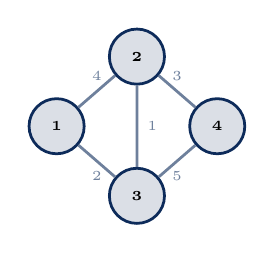
\begin{tikzpicture}[scale=0.68,
          no/.style={circle,draw=gemaBlue,fill=gemaBlue!15,
                     minimum size=7mm,font=\bfseries\tiny,line width=1pt}]
          \node[no] (1) at (0,1.5) {1};
          \node[no] (2) at (1.5,2.8) {2};
          \node[no] (3) at (1.5,0.2) {3};
          \node[no] (4) at (3.0,1.5) {4};
          \draw[gemaBlue!60,line width=1pt]
            (1)--(2) node[midway,above,font=\tiny]{4}
            (1)--(3) node[midway,below,font=\tiny]{2}
            (2)--(4) node[midway,above,font=\tiny]{3}
            (3)--(4) node[midway,below,font=\tiny]{5}
            (2)--(3) node[midway,right,font=\tiny]{1};
        \end{tikzpicture}\\[3pt]
        Inicio=1: dist=[0,4,2,6]\\
        Menor: 1$\to$3$\to$2$\to$4
      \end{tcolorbox}
      \vspace{0.1cm}
      \begin{tcolorbox}[caixaVermelho,title={Cuidado}]
        \footnotesize
        A PQ pode ter entradas\\
        desatualizadas. Sempre\\
        verifique: \texttt{if (d > dist[v]) continue;}
      \end{tcolorbox}
  \end{columns}
\end{frame}

% ─────────────────────────────────────────────────────────────
%  COMPARAÇÃO FINAL
% ─────────────────────────────────────────────────────────────
\begin{frame}{Queue vs.\ Priority Queue --- Quando Usar Cada Uma?}
  \begin{tcolorbox}[caixaAzul,title={Tabela Comparativa Completa}]
    \centering\small
    \begin{tabular}{lll}
      \toprule
      \textbf{Criterio} & \textbf{Queue} & \textbf{Priority Queue}\\
      \midrule
      Ordem de saida & Chegada (FIFO) & Prioridade (maior/menor)\\
      push           & O(1) & O(log n)\\
      pop            & O(1) & O(log n)\\
      peek           & O(1) --- \texttt{front()} & O(1) --- \texttt{top()}\\
      Header STL     & \texttt{<queue>} & \texttt{<queue>}\\
      Declaracao     & \texttt{queue<T>} & \texttt{priority\_queue<T,...>}\\
      \midrule
      Algoritmo tipico & BFS, simulacoes & Dijkstra, agendamento\\
      Pergunta-chave & ``Chegou primeiro?'' & ``E mais importante?''\\
      \bottomrule
    \end{tabular}
  \end{tcolorbox}
  \vspace{0.15cm}
  \begin{columns}[t]
    \column{0.47\textwidth}
      \begin{tcolorbox}[caixaLaranja,title={Use Queue quando...}]
        \begin{itemize}\small
          \item A ordem de chegada importa
          \item Fazer BFS em grafo/grade
          \item Simular uma fila real
          \item Processar eventos em sequencia
        \end{itemize}
      \end{tcolorbox}
    \column{0.50\textwidth}
      \begin{tcolorbox}[caixaRoxa,title={Use Priority Queue quando...}]
        \begin{itemize}\small
          \item Precisa do maior ou menor elemento rapido
          \item Implementar Dijkstra, Prim, A*
          \item Agendamento de tarefas por urgencia
          \item Mesclar listas ordenadas
        \end{itemize}
      \end{tcolorbox}
  \end{columns}
\end{frame}

% ─────────────────────────────────────────────────────────────
%  EXERCÍCIO PRÁTICO
% ─────────────────────────────────────────────────────────────
\begin{frame}[fragile,shrink=5]{Exercicio Pratico --- Estilo OBI}
  \begin{tcolorbox}[caixaRoxa,title={Problema: Hospital de Campanha}]
    \small
    Um hospital tem $Q$ pacientes chegando ao longo do dia.
    Cada paciente tem uma \textbf{gravidade} (inteiro de 1 a 10).
    O hospital atende sempre o paciente de \textbf{maior gravidade} disponivel.
    Dado o log de eventos: \texttt{E g} (chega paciente com gravidade g)
    ou \texttt{A} (atende o mais grave), imprima a gravidade de cada atendimento
    ou \texttt{-1} se a fila estiver vazia.\\[4pt]
    \textbf{Entrada:} \texttt{5 | E 3 | E 7 | E 1 | A | A}
    \quad\textbf{Saida:} \texttt{7\ \ 3}
  \end{tcolorbox}
  \vspace{0.1cm}
  \begin{columns}[t]
    \column{0.52\textwidth}
      \begin{tcolorbox}[caixaCodigo]
        \begin{lstlisting}[style=cppsmall]
#include <bits/stdc++.h>
using namespace std;

int main(){
    int Q; cin >> Q;
    priority_queue<int> pq; // max-heap

    while(Q--){
        char op; cin >> op;
        if(op == 'E'){
            int g; cin >> g;
            pq.push(g);       // novo paciente
        } else {
            if(pq.empty())
                cout << -1 << "\n";
            else {
                cout << pq.top() << "\n";
                pq.pop();     // atende o mais grave
            }
        }
    }
    return 0;
}
        \end{lstlisting}
      \end{tcolorbox}
    \column{0.45\textwidth}
      \begin{tcolorbox}[caixaAmarelo,title={Estrategia de solucao}]
        \footnotesize
        \textbf{1. Identificar a estrutura:}\\
        Preciso do \textbf{maior elemento}\\
        rapidamente $\to$ Max-Heap!\\[5pt]
        \textbf{2. Modelar:}\\
        Evento E $\to$ \texttt{push}\\
        Evento A $\to$ \texttt{top} + \texttt{pop}\\[5pt]
        \textbf{3. Tratar borda:}\\
        Fila vazia ao atender $\to$ \texttt{-1}\\[5pt]
        \textbf{Complexidade:}\\
        O(Q log Q)
      \end{tcolorbox}
      \vspace{0.15cm}
      \begin{tcolorbox}[caixaVerde,title={Variacao: fila normal}]
        \footnotesize
        Se o enunciado dissesse\\
        ``atende por ordem de\\
        chegada'' $\to$ use \texttt{queue}\\
        com \texttt{front()} no lugar\\
        de \texttt{top()}.
      \end{tcolorbox}
  \end{columns}
\end{frame}

% ─────────────────────────────────────────────────────────────
%  COMO IDENTIFICAR NA PROVA
% ─────────────────────────────────────────────────────────────
\begin{frame}{Como Identificar na Prova?}
  \begin{columns}[t]
    \column{0.47\textwidth}
      \begin{block}{Palavras-chave para Queue}
        \begin{itemize}\small
          \item ``menor caminho em passos'' (BFS)
          \item ``nivel a nivel'', ``onda''
          \item ``fila de processamento''
          \item ``propaga para vizinhos''
          \item ``labirinto'', ``grade'', ``distancia minima''
          \item ``primeiro a chegar, primeiro a sair''
        \end{itemize}
      \end{block}
      \vspace{0.15cm}
      \begin{tcolorbox}[caixaLaranja,title={Sinal: use Queue}]
        \small
        Problema em \textbf{grade/grafo} sem
        pesos (ou pesos iguais) e precisa
        de \textbf{menor distancia}.
      \end{tcolorbox}
    \column{0.50\textwidth}
      \begin{block}{Palavras-chave para Priority Queue}
        \begin{itemize}\small
          \item ``maior prioridade'', ``mais urgente''
          \item ``menor custo'', ``menor distancia'' (com pesos)
          \item ``$k$-esimo maior/menor''
          \item ``processar em ordem de importancia''
          \item ``Dijkstra'', ``Prim'', ``A*''
          \item ``agendamento'', ``escalonamento''
        \end{itemize}
      \end{block}
      \vspace{0.15cm}
      \begin{tcolorbox}[caixaRoxa,title={Sinal: use Priority Queue}]
        \small
        Problema em grafo com \textbf{pesos}
        e precisa de \textbf{menor caminho},
        ou precisa do \textbf{max/min rapido}.
      \end{tcolorbox}
  \end{columns}
  \vspace{0.1cm}
  \begin{tcolorbox}[caixaAmarelo,title={Pergunta magica}]
    \small
    \textbf{A ordem de chegada importa?} $\to$ Queue (FIFO)\\
    \textbf{O valor/prioridade importa?} $\to$ Priority Queue (Heap)\\
    \textbf{A ordem de saida importa (do mais recente)?} $\to$ Stack (LIFO)
  \end{tcolorbox}
\end{frame}

% ─────────────────────────────────────────────────────────────
%  RESUMO GERAL
% ─────────────────────────────────────────────────────────────
\begin{frame}[shrink=5]{Resumo Geral}
  \begin{columns}[t]
    \column{0.31\textwidth}
      \begin{block}{Stack (Aula 02)}
        \begin{itemize}\footnotesize
          \item LIFO
          \item push/pop/top: O(1)
          \item DFS, expressoes,\\parenteses
          \item \texttt{stack<T>}
        \end{itemize}
      \end{block}
    \column{0.31\textwidth}
      \begin{block}{Queue (Hoje)}
        \begin{itemize}\footnotesize
          \item FIFO
          \item push/pop/front: O(1)
          \item BFS, simulacoes,\\filas de processamento
          \item \texttt{queue<T>}
        \end{itemize}
      \end{block}
    \column{0.31\textwidth}
      \begin{block}{Priority Queue (Hoje)}
        \begin{itemize}\footnotesize
          \item Por prioridade
          \item push/pop: O(log n)\\top: O(1)
          \item Dijkstra, agendamento,\\top-k elementos
          \item \texttt{priority\_queue<T,...>}
        \end{itemize}
      \end{block}
  \end{columns}
  \vspace{0.15cm}
  \begin{columns}[t]
    \column{0.47\textwidth}
      \begin{tcolorbox}[caixaVerde,title={Problemas para Praticar}]
        \footnotesize
        \textbf{Queue (BFS):}
        \begin{itemize}
          \item CF 1321B --- Joystick (BFS)
          \item CF 652E --- Enumerating Substrings
          \item NEPS --- Labirinto Minimo
        \end{itemize}
        \textbf{Priority Queue:}
        \begin{itemize}
          \item CF 20C --- Histogram (heap interno)
          \item CF 797C --- Minimal string (greedy + PQ)
          \item NEPS --- Dijkstra classico
        \end{itemize}
      \end{tcolorbox}
    \column{0.50\textwidth}
      \begin{tcolorbox}[caixaAzul,title={Template Mental}]
        \small
        \textbf{BFS:}\\
        \texttt{queue<int> q; q.push(s);}\\
        \texttt{while(!q.empty())\{v=q.front();q.pop();\}}\\[6pt]
        \textbf{Dijkstra:}\\
        \texttt{priority\_queue<pii,vector<pii>,}\\
        \texttt{greater<pii>> pq;}\\
        \texttt{pq.push(\{0, inicio\});}\\[6pt]
        \textbf{Max-element rapido:}\\
        \texttt{priority\_queue<int> pq;}\\
        \texttt{pq.top(); // sempre o maior}
      \end{tcolorbox}
  \end{columns}
\end{frame}

% ─────────────────────────────────────────────────────────────
%  SLIDE FINAL
% ─────────────────────────────────────────────────────────────
{
\setbeamertemplate{footline}{}
\begin{frame}[noframenumbering]
  \centering
  \vspace{0.1cm}
  \begin{columns}[c]
    \column{0.30\textwidth}
      \centering
      
\includegraphics[width=0.65\linewidth]{logo.png}
    \column{0.38\textwidth}
      \centering
      {\large\color{gemaBlue}\bfseries Bons estudos\\e boa prova!}\par
      \vspace{0.15cm}
      {\small\color{gemaCyan} GEMA --- Maratonas de Programacao}\par
      \vspace{0.2cm}
      {\footnotesize\color{gray} Proxima aula: Grafos e BFS/DFS avancado}
    \column{0.30\textwidth}
      \centering
      
\includegraphics[width=0.65\linewidth]{logo_obi.png}
  \end{columns}
  \vspace{0.25cm}
  \begin{tcolorbox}[caixaAzul,title={Dica de Ouro para Competicoes},
      width=0.80\textwidth]
    \centering\small
    \textbf{Regra das 3 perguntas:}\\[5pt]
    ``Preciso do mais recente?'' $\to$ \textbf{Stack}\\
    ``Preciso do mais antigo?'' $\to$ \textbf{Queue}\\
    ``Preciso do mais importante?'' $\to$ \textbf{Priority Queue}
  \end{tcolorbox}
  \vspace{0.2cm}
  \begin{tcolorbox}[caixaVerde,title={},width=0.78\textwidth]
    \centering\small
    \textbf{Pratique:} \texttt{codeforces.com} $\cdot$ \texttt{neps.com.br}
    $\cdot$ \texttt{br.spoj.com}\\[3pt]
    \textbf{Estude:} cp-algorithms.com $\cdot$ USACO Guide $\cdot$ CSES Problemset
  \end{tcolorbox}
  \vspace{0.15cm}
  {\small\color{gray}\itshape
    ``Estruturas de dados sao a alma dos algoritmos eficientes.''}
\end{frame}
}

\end{document}